% ============================================================
%  PAPERS_COMPARISON_SLIDES.tex
%  Slide version of PAPERS_COMPARISON_REPORT: the seven papers in papers/
%  compared with the baseline (Daga et al. 2026, Sci. Rep. 16:26840), checks
%  of their printed numbers, and the gaps with possible fixes.
%  Figures and matrix tables come from reimplementation/papers_consistency_checks.py.
%  Compile from latex_report/:  ..\tectonic_bin\tectonic.exe PAPERS_COMPARISON_SLIDES.tex
% ============================================================
\documentclass[aspectratio=169,10pt,t,xcolor={table}]{beamer}
\usetheme{Madrid}
\usepackage{amsmath,amssymb}
\usepackage{booktabs,array,tabularx}
\usepackage{graphicx}
\usepackage{adjustbox}
\usepackage{tikz}
\usetikzlibrary{positioning,arrows.meta}
\graphicspath{{../reimplementation/figures/}}
\newcommand{\tabdir}{../reimplementation/tex/papers/}

\definecolor{qnavy}{HTML}{1B3A5C}
\definecolor{qteal}{HTML}{0E7C7B}
\definecolor{qred}{HTML}{B23A3A}
\definecolor{qgreen}{HTML}{2E7D4F}
\definecolor{qamber}{HTML}{C9821B}
\definecolor{qlight}{HTML}{EEF3F8}
\definecolor{okbg}{RGB}{214,240,222}
\definecolor{warnbg}{RGB}{252,236,200}
\definecolor{badbg}{RGB}{248,214,214}
\setbeamercolor{structure}{fg=qnavy}
\setbeamercolor{palette primary}{bg=qnavy,fg=white}
\setbeamercolor{palette secondary}{bg=qteal,fg=white}
\setbeamercolor{palette tertiary}{bg=qnavy,fg=white}
\setbeamercolor{frametitle}{bg=qnavy,fg=white}
\setbeamercolor{title}{bg=qnavy,fg=white}
\setbeamercolor{block title}{bg=qnavy,fg=white}
\setbeamercolor{block body}{bg=qlight,fg=black}
\setbeamercolor{block title alerted}{bg=qred,fg=white}
\setbeamercolor{block body alerted}{bg=qred!7,fg=black}
\setbeamercolor{block title example}{bg=qteal,fg=white}
\setbeamercolor{block body example}{bg=qteal!8,fg=black}
\setbeamercolor{item}{fg=qteal}
\setbeamertemplate{navigation symbols}{}
\setbeamertemplate{itemize items}[circle]
\setbeamertemplate{enumerate items}[default]
\setbeamerfont{frametitle}{size=\large,series=\bfseries}
\setbeamertemplate{caption}{\raggedright\insertcaption\par}
\setbeamertemplate{section page}{%
  \begin{centering}\vspace{2.6cm}
  {\usebeamercolor[fg]{structure}\LARGE\bfseries\insertsection\par}
  \end{centering}}
\AtBeginSection{\frame[plain]{\sectionpage}}

\newcommand{\ok}[1]{\textcolor{qgreen}{\textbf{#1}}}
\newcommand{\bad}[1]{\textcolor{qred}{\textbf{#1}}}
\newcommand{\warn}[1]{\textcolor{qamber}{\textbf{#1}}}
\newcommand{\code}[1]{\texttt{\small #1}}
\newcommand{\src}[1]{{\tiny\textcolor{gray}{#1}}}
\newcolumntype{L}[1]{>{\raggedright\arraybackslash}p{#1}}
\newcolumntype{Y}{>{\raggedright\arraybackslash}X}

\title[Seven papers vs the baseline]{The seven papers in \texttt{papers/} compared with the baseline}
\subtitle{Daga et al.\ (2026), \emph{Sci.\ Rep.}\ 16:26840: what each paper did, which printed numbers hold up, and the gaps with fixes}
\author[M.~Wajahat]{Prepared for M.~Wajahat}
\institute[]{Repository \texttt{Adaptive-Quantum-Kernel-Selection}; full report: \texttt{PAPERS\_COMPARISON\_REPORT.pdf}}
\date{20 October 2026}

\begin{document}

\begin{frame}[plain]
\titlepage
\end{frame}

\begin{frame}{Roadmap}
\begin{columns}[T]
\column{0.53\textwidth}
\begin{enumerate}
  \item \textbf{Ground rules}: what was read, what was checked, what was not.
  \item \textbf{The baseline}: what Daga et al.\ did and what the re-implementation showed.
  \item \textbf{The seven papers}, one by one: method, results, checks, relation to the baseline.
  \item \textbf{Side by side}: Pima, breast cancer, kernel mechanics, balanced metrics.
  \item \textbf{Three-way}: baseline paper vs re-implementation vs the seven papers.
  \item \textbf{Practices and gaps}, with fixes.
  \item \textbf{Priorities} and what could not be checked.
\end{enumerate}
\column{0.44\textwidth}
\begin{block}{One-line answer}
No paper shows a quantum model beating a classical one with statistical support. The baseline has the best evaluation of the eight, but still has measurable gaps. Three comparison papers print numbers that fail simple arithmetic.
\end{block}
\begin{exampleblock}{Reading guide}
\ok{green} = holds; \warn{amber} = partly or unclear; \bad{red} = contradicted by the paper's own numbers. Check IDs such as \texttt{[P4-1]} refer to the report's Appendix A.
\end{exampleblock}
\end{columns}
\end{frame}

% ============================================================
\section{Ground rules}
% ============================================================
\begin{frame}{How the comparison was made}
\begin{columns}[T]
\column{0.5\textwidth}
\begin{block}{Every number is one of three kinds}
\begin{itemize}
  \item \textbf{Printed}: quoted from a paper with its page. A script re-finds each transcribed value in the PDF text of that page: \ok{180 of 180 found}.
  \item \textbf{Computed}: arithmetic on printed numbers (F1 from precision and recall, kappa bounds, AUC bound from a confusion matrix, Wilson intervals, G-mean).
  \item \textbf{Re-implementation}: this repository's rerun of the baseline on Pima Diabetes.
\end{itemize}
\end{block}
\column{0.46\textwidth}
\begin{alertblock}{What was not done}
\begin{itemize}
  \item None of the seven papers' code was run and none of their models was re-trained.
  \item So the slides judge what the papers \emph{report} and whether it is internally consistent, not whether it reproduces.
  \item Numbers that exist only inside figures were read at full resolution and are labelled ``from a figure''.
\end{itemize}
\end{alertblock}
\src{Script: reimplementation/papers\_consistency\_checks.py; log: results/papers\_comparison/text\_log.json}
\end{columns}
\end{frame}

\begin{frame}{The baseline and the seven papers}
\centering\scriptsize
\begin{tabularx}{\textwidth}{c L{3.7cm} L{3.0cm} Y L{2.7cm} c}
\toprule
Tag & Paper & Venue & Data & Quantum part & Cited by B \\
\midrule
B & Daga, Naole, Parikh, Bommineni, Ramu & Sci.\ Rep.\ 16:26840 (2026) & Parkinson's 195, WDBC 569, Pima 768 & 3 fidelity kernels, simulated & -- \\
P1 & Upama, Haque, Alam, Ahamed & Mach.\ Learn.\ Appl.\ 24 (2026) & Early-stage diabetes 520; Pima 768 & QSVM simulated; ``QRF'' classical & no \\
P2 & Young II (QISICGM) & arXiv:2509.12259 (2025) & Pima + 2,000 synthetic rows & quantum-inspired, classical & ref.\ 15 \\
P3 & Kotha et al.\ (DiaBeats) & IEEE I3CTCON (2026) & Pima 768 & none & no \\
P4 & Chitra Kiran N et al.\ (HQCAN) & IEEE ICICI (2025) & Pima 768 (IoT claimed) & ``4 qubits'', not described & ref.\ 22 \\
P5 & Yadav, Sheoran, Sheoran & PeerJ CS 12:e3600 (2026) & WDBC 569 & Z/ZZ kernels + QNN, simulated & ref.\ 13 \\
P6 & Sodar, Murthy, Jonnalagadda, Cherukuri & EPJ Quantum Technol.\ 13:17 (2026) & two encrypted-traffic datasets & QSVM, QKNN, hybrid, simulated & ref.\ 19 \\
P7 & Zhang, Cheng, Xue, Wu, Zhang (DeSCN-GIF) & IEEE TFS 33(9) (2025) & 5 voice datasets, depression & none & ref.\ 8 \\
\midrule
R & re-implementation of B (this repository) & -- & Pima 768 only & B's 3 kernels, simulated & -- \\
\bottomrule
\end{tabularx}
\par\smallskip\raggedright\scriptsize
Four papers share the baseline's Pima data (P1--P4), one shares its breast cancer data with quantum kernels (P5), one shares its kernel construction (P6), one shares its clinical imbalance problem (P7). R is compared with all of them in Part 5.
\end{frame}

\begin{frame}{Findings at a glance}
\footnotesize
\begin{enumerate}
  \item \textbf{No quantum win with support.} Same data, same split: B at parity; P1's QSVM 0.65 vs RF 0.76 on Pima; P5's best hybrid 0.956 vs its own SVM 0.9737; P6's pure quantum models below classical in 8 of 8.
  \item \textbf{The baseline has the most complete evaluation} (10 of 12 practices; next best P7 with 7.5).
  \item \textbf{The baseline still has measurable gaps}: fold-local preprocessing drops its Diabetes stacking from 0.766 to 0.746; untrained VQC; mismatched noise reference; untuned baselines.
  \item \bad{P4: impossible numbers} (F1 above both precision and recall; kappa above accuracy; four accuracies).
  \item \bad{P3: AUC 1.00 ruled out by its own confusion matrix} (AUC $\le$ 0.970).
  \item \bad{P2: synthetic rows in every test fold}; class counts do not add up; text and figure disagree.
  \item \warn{P5: two feature maps, not three}; ``t-test values'' are timings; recall is benign recall.
  \item \warn{Breast cancer ``recall'' is benign recall in both B and P5.}
  \item \textbf{Shared gaps}: no external or person-level validation anywhere; no hardware anywhere.
  \item \textbf{What transfers}: P7's statistics, P5's hold-out, P2's probability meta-features, P6's hybrid baseline.
  \item \textbf{Three-way}: R reproduces B exactly; B's recall gain survives leakage-free preprocessing, its accuracy gain does not; R's leakage-free numbers are the most rigorous Pima results in the set.
\end{enumerate}
\end{frame}

% ============================================================
\section{The baseline: Daga et al.\ (2026)}
% ============================================================
\begin{frame}{What the baseline does}
\begin{center}
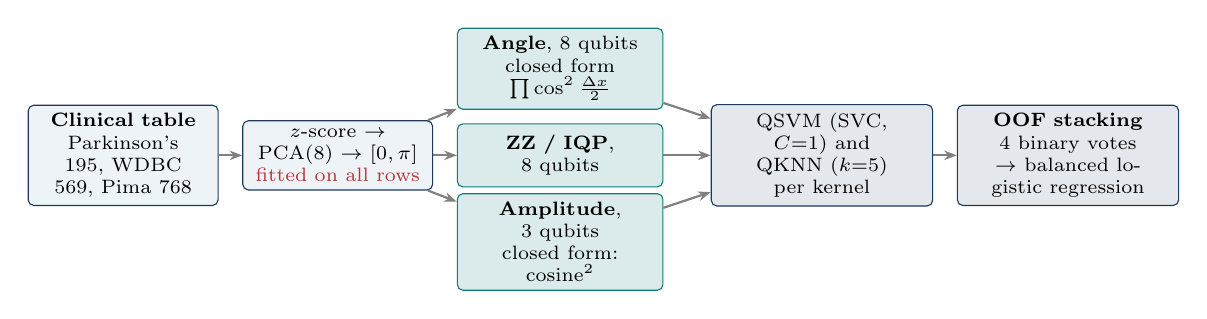
\begin{tikzpicture}[font=\scriptsize, node distance=3mm,
  box/.style={draw, rounded corners=2pt, align=center, inner sep=3pt, minimum height=8mm},
  d/.style={box, fill=qlight, draw=qnavy, text width=2.2cm},
  q/.style={box, fill=qteal!15, draw=qteal, text width=2.4cm},
  e/.style={box, fill=qnavy!12, draw=qnavy, text width=2.6cm},
  arr/.style={-{Stealth[length=1.6mm]}, thick, gray}]
\node[d] (data) {\textbf{Clinical table}\\Parkinson's 195, WDBC 569, Pima 768};
\node[d, right=of data] (prep) {$z$-score $\to$ PCA(8) $\to$ $[0,\pi]$\\\textcolor{qred}{fitted on all rows}};
\node[q, right=of prep, yshift=11mm] (ang) {\textbf{Angle}, 8 qubits\\closed form $\prod\cos^2\frac{\Delta x}{2}$};
\node[q, right=of prep] (zz) {\textbf{ZZ / IQP}, 8 qubits};
\node[q, right=of prep, yshift=-11mm] (amp) {\textbf{Amplitude}, 3 qubits\\closed form: cosine$^2$};
\node[e, right=of zz, xshift=3mm] (base) {QSVM (SVC, $C{=}1$) and\\QKNN ($k{=}5$) per kernel};
\node[e, right=of base] (st) {\textbf{OOF stacking}\\4 binary votes $\to$ balanced logistic regression};
\draw[arr] (data) -- (prep);
\draw[arr] (prep) -- (ang); \draw[arr] (prep) -- (zz); \draw[arr] (prep) -- (amp);
\draw[arr] (ang) -- (base); \draw[arr] (zz) -- (base); \draw[arr] (amp) -- (base);
\draw[arr] (base) -- (st);
\end{tikzpicture}
\end{center}
\begin{columns}[T]
\column{0.5\textwidth}
\footnotesize
\begin{itemize}
  \item 10-fold outer, 5-fold inner CV, seed 42; 1,000-resample bootstrap intervals; McNemar tests.
  \item Ablation, calibration, SHAP/LIME/permutation, PCA backtracking, depolarizing noise, VQC, XGBoost/RF/classical stacker. Code on GitHub.
\end{itemize}
\column{0.47\textwidth}
\scriptsize
\begin{tabular}{lll}
\toprule
Dataset & Headline (abstract, p.~1) & \\
\midrule
Parkinson's & specificity 0.585 $\to$ 0.813 & $p<0.001$ \\
WDBC & accuracy 0.970 vs 0.964 & all $p>0.05$ \\
Pima & recall 0.553 $\to$ 0.621 & $p=0.004$ \\
All & VQC ROC-AUC 0.51--0.57 & \\
\bottomrule
\end{tabular}
\end{columns}
\end{frame}

\begin{frame}{What the re-implementation established on Pima Diabetes}
\centering\scriptsize
\begin{tabularx}{\textwidth}{L{3.6cm} Y L{2.6cm}}
\toprule
Item & Re-implementation & Verdict \\
\midrule
Bootstrap table (Table 9) & 108 of 108 values identical to the printed digits & \ok{exact} \\
Ablation, McNemar, calibration, XAI, backtracking & identical to the printed digits & \ok{exact} \\
Recall gain 0.553 $\to$ 0.621 & ahead in 10/10 seeds; Holm $p$ = 0.035 ($10^4$ resamples), 0.112 (paper's 1,000), 0.204 (parametric) & \warn{robust direction, fragile significance} \\
Accuracy gain 0.758 $\to$ 0.766 & ahead in 6/10 seeds, mean $+0.001$; paper's own McNemar $p=0.556$ & \warn{parity} \\
Preprocessing inside the folds & stacking 0.766 $\to$ \textbf{0.746}; RBF-SVM 0.758 $\to$ 0.759 & \bad{gain disappears} \\
Tuned classical baselines & RBF-SVM 0.760, XGBoost 0.759 (McNemar vs stacking $p$ = 0.72, 0.69) & \warn{parity} \\
VQC & released loss has zero gradient: an untrained random circuit & \bad{baseline invalid} \\
Noise study (Table 19) & 0\,\% row uses a chain kernel; with the benchmark kernel, 10\,\% degradation is +0.117 / +0.167 & \bad{wrong reference} \\
\bottomrule
\end{tabularx}
\par\smallskip\src{Source: reimplementation/results/diabetes/ (see DIABETES\_REIMPLEMENTATION\_REPORT\_v2.pdf)}
\end{frame}

\begin{frame}{How the baseline describes the five papers it cites}
\centering\scriptsize
\begin{tabularx}{\textwidth}{c L{4.0cm} Y L{2.8cm}}
\toprule
Ref. & Baseline says & Full paper shows & Consequence \\
\midrule
8 (P7) & classical deep ensemble for imbalanced depression data & correct; P7 also has 100 repeated splits, tuned baselines, Friedman--Nemenyi & \ok{accurate} \\
13 (P5) & hybrid QSVM$\to$QNN, ``over 95\,\%'' & 95.61\,\% correct, but P5's own SVM and logistic regression reach 97.37\,\% & \warn{incomplete} \\
15 (P2) & classical, ``no true Hilbert space''; F1 0.8933 & correct, but synthetic rows sit in the test folds; and two of B's own kernels are closed-form classical & \warn{contrast weaker than stated} \\
19 (P6) & QSVM/QKNN ``competitive'' on cybersecurity data & only the hybrids are; pure QSVM/QKNN (B's design) lose 8 of 8 & \warn{misattributed} \\
22 (P4) & 99.7\,\% accuracy; overfitting concerns & one of four accuracies, beside an impossible F1 and kappa & \bad{should not be cited} \\
\bottomrule
\end{tabularx}
\end{frame}

% ============================================================
\section{The seven papers}
% ============================================================
\begin{frame}{P1 \quad Upama et al.\ (2026): causal inference + quantum ML for diabetes}
\begin{columns}[T]
\column{0.5\textwidth}
\begin{block}{What they did}
\footnotesize
\begin{itemize}
  \item Early-stage diabetes questionnaire, 520 records (320/200), 16 features; causal LinearDML keeps 10.
  \item Linear SVM, QSVM (Qiskit ZZFeatureMap, statevector), RF (100 trees), ``QRF'' = \emph{a regular RF with capped depth}.
  \item Same pipeline on Pima with 7 features.
\end{itemize}
\end{block}
\begin{block}{What they report}
\footnotesize
Test set of 104: SVM 0.9231, RF 0.9712, QSVM 0.9712, ``QRF'' 0.9615.\\
Pima: SVM 72\,\%, \textbf{QSVM 65\,\%}, RF 76\,\%, ``QRF'' 72\,\%.
\end{block}
\column{0.46\textwidth}
\begin{alertblock}{Checks}
\footnotesize
\begin{itemize}
  \item QSVM vs SVM = 101 vs 96 of 104. Even if all 5 disagreements favour the QSVM, exact McNemar $p=0.0625$. \texttt{[P1-3]}
  \item ``QRF'' contains no quantum computation. \texttt{[P1-2]}
  \item Causal feature selection runs on all data before the split.
\end{itemize}
\end{alertblock}
\begin{exampleblock}{Relation to B}
\footnotesize
Same Pima rows, opposite picture: B's QSVM-ZZ 0.759 = its RBF-SVM; P1's QSVM is its worst model. Different features, library and protocol, so not rankable. Not cited by B.
\end{exampleblock}
\end{columns}
\end{frame}

\begin{frame}{P2 \quad Young (2025): QISICGM quantum-inspired stack}
\begin{columns}[T]
\column{0.5\textwidth}
\begin{block}{What they did}
\footnotesize
\begin{itemize}
  \item Pima + 2,000 GMM synthetic rows ``fitted to the minority class'': 2,768 rows, 1,949 positive.
  \item Phase feature map, concept graph, sequence model: all classical.
  \item RF, ET, transformer, CNN, FFNN $\to$ isotonic calibration $\to$ logistic-regression meta-learner, 5-fold OOF. Code on GitHub.
\end{itemize}
\end{block}
\begin{block}{What they report}
\footnotesize
OOF F1 0.8933, AUC 0.8699, Brier 0.12. Baselines quoted from other papers: RF F1 0.821, XGBoost 0.854.
\end{block}
\column{0.46\textwidth}
\begin{exampleblock}{Relation to B}
\footnotesize
\begin{itemize}
  \item The closest architecture to B: stacked base models + logistic-regression meta-learner on out-of-fold outputs.
  \item P2 feeds calibrated probabilities to the meta-learner, which B lists as future work.
  \item B dismisses P2 for having ``no true Hilbert space'', but two of B's three kernels are closed-form classical functions too.
  \item Not comparable numerically: P2 reports F1 on augmented data.
\end{itemize}
\end{exampleblock}
\end{columns}
\end{frame}

\begin{frame}{P2 checks: the numbers do not hold together}
\begin{columns}[T]
\column{0.5\textwidth}
\begin{alertblock}{Arithmetic}
\footnotesize
\begin{itemize}
  \item 268 real + 2,000 synthetic positives = \textbf{2,268}, not 1,949. \texttt{[P2-1]}
  \item With 70\,\% positives, ``always diabetic'' scores \textbf{F1 = 0.826}. \texttt{[P2-2]}
  \item Synthetic rows are created before the folds, so every test fold contains them. \texttt{[P2-6]}
\end{itemize}
\end{alertblock}
\column{0.46\textwidth}
\begin{alertblock}{Text vs its own Fig.~1 (from a figure)}
\scriptsize
\begin{tabular}{lll}
\toprule
 & Text (p.~7) & Fig.~1 \\
\midrule
Meta F1 range & 0.881--0.902 & 0.8849--0.9123 \\
Meta AUC range & 0.852--0.885 & 0.8281--0.8989 \\
RF F1 & 0.845 & 0.8950 \\
ET F1 & 0.852 & 0.8948 \\
Own RF F1 / AUC & -- & 0.8950 / 0.8046 \\
Meta F1 (average) & 0.8933 & 0.8962 \\
\bottomrule
\end{tabular}
\par\smallskip\footnotesize
Against its \emph{own} RF the F1 gain is \textbf{0.001}; the 0.07 gain in the text uses other papers' numbers. \texttt{[P2-3..5]}
\end{alertblock}
\end{columns}
\end{frame}

\begin{frame}{P3 \quad Kotha et al.\ (2026): DiaBeats web system}
\begin{columns}[T]
\column{0.48\textwidth}
\begin{block}{What they did}
\footnotesize
Random forest on Pima; zeros replaced by non-zero medians; z-scores; Flask + Streamlit app with adjustable threshold. No quantum part; cites P2; not cited by B.
\end{block}
\begin{block}{What they report}
\footnotesize
\textbf{No numbers in the text.} Figures only: ROC ``AUC = 1.00'', confusion matrix TN 90, FP 10, FN 15, TP 35, feature importances.
\end{block}
\column{0.48\textwidth}
\begin{alertblock}{Checks (from figures)}
\footnotesize
\begin{itemize}
  \item Matrix gives $n=150$, accuracy \textbf{0.833} [0.766, 0.884], recall 0.700, specificity 0.900. \texttt{[P3-1, P3-5]}
  \item 15 FN $\times$ 10 FP = 150 of 5,000 pairs mis-ordered: \textbf{AUC $\le$ 0.970}, so 1.00 is impossible for the same predictions. \texttt{[P3-2]}
  \item ``Summarized in Table I'' points to the attribute table; text ranks insulin high, figure ranks it last. \texttt{[P3-3, P3-4]}
\end{itemize}
\end{alertblock}
\end{columns}
\end{frame}

\begin{frame}{P4 \quad Chitra Kiran N et al.\ (2025): HQCAN-BSTOA}
\begin{columns}[T]
\column{0.48\textwidth}
\begin{block}{What they did}
\footnotesize
\begin{itemize}
  \item Described as IoT wearable monitoring; experiments use only Pima, one 80/20 split.
  \item Guided filtering $\to$ scale-aware transformer $\to$ ``hybrid quantum--classical adversarial network'' (4 qubits, 200 epochs) tuned by a sooty tern optimiser.
  \item Quantum circuit not described; the reference for HQCAN (ref.\ 13) is a power-electronics paper on a LUO converter.
\end{itemize}
\end{block}
\column{0.48\textwidth}
\begin{block}{What they report}
\scriptsize
\begin{tabular}{ll}
\toprule
Where & Accuracy \\
\midrule
Abstract (p.~1) & 99.7\,\% \\
Results (p.~4) & 99.5\,\% \\
 & (precision 99.5, recall 99.3, F1 99.6) \\
Test curve (p.~5) & 98.9\,\% \\
Conclusion (p.~5) & 99.8\,\% \\
Table IV & kappa 99.7\,\% \\
 & (RMSE 4\,\%, MAE 1.04\,\%) \\
\bottomrule
\end{tabular}
\end{block}
\footnotesize B cites the 99.7\,\% as a result (ref.\ 22).
\end{columns}
\end{frame}

\begin{frame}{P4 checks: arithmetically impossible}
\begin{columns}[T]
\column{0.5\textwidth}
\begin{alertblock}{F1 outside its own range \texttt{[P4-1]}}
\footnotesize
F1 is the harmonic mean of precision and recall, so it lies between them.\\
$P=0.995$, $R=0.993$ $\Rightarrow$ F1 $=0.994$, \textbf{not 0.996}.
\end{alertblock}
\begin{alertblock}{Kappa above accuracy \texttt{[P4-2]}}
\footnotesize
Kappa $\le$ accuracy whenever accuracy $<1$.\\
Largest kappa with the Pima class mix: 0.976, 0.989, 0.993, 0.996 at the four printed accuracies. \textbf{0.997 fits none.}
\end{alertblock}
\column{0.46\textwidth}
\begin{alertblock}{More contradictions}
\footnotesize
\begin{itemize}
  \item ``Error rate of 4\,\%'' next to 99.5\,\% accuracy. \texttt{[P4-3]}
  \item Four accuracies for one model and one split. \texttt{[P4-4]}
  \item ``768 female patients with diabetes, up to 21 years old''; its own Table III says 268 with diabetes, and Pima participants are 21 or older. \texttt{[P4-5]}
  \item Baselines with kappa 99.0--99.4\,\% next to accuracy bars below 95\,\%.
\end{itemize}
\end{alertblock}
\begin{block}{Consequence}
\footnotesize No P4 number should be used as a result.
\end{block}
\end{columns}
\end{frame}

\begin{frame}{P5 \quad Yadav, Sheoran, Sheoran (2026): hybrid QSVM$\to$QNN on WDBC}
\begin{columns}[T]
\column{0.5\textwidth}
\begin{block}{What they did}
\footnotesize
\begin{itemize}
  \item WDBC; 7 features; 80/20 stratified split $\to$ 114-record hold-out; 5-fold CV $\times$ 3 seeds.
  \item QSVM with Qiskit fidelity kernels: Z, ZZ, ``Pauli'' (7 qubits, 1 rep).
  \item Hybrid: QSVM margin + 1 PCA component $\to$ 2-qubit QNN (COBYLA).
  \item Classical baselines with nested CV (5 $\times$ 3). Code on Zenodo.
\end{itemize}
\end{block}
\column{0.46\textwidth}
\begin{block}{What they report (hold-out accuracy)}
\scriptsize
\begin{tabular}{lccc}
\toprule
 & Z & ZZ & Pauli \\
\midrule
QSVM & 0.947 & 0.860 & 0.860 \\
QNN & 0.605 & 0.491 & 0.544 \\
Hybrid & 0.947--0.956 & 0.833--0.860 & 0.947--0.956$^{*}$ \\
\bottomrule
\end{tabular}
\par{\tiny $^{*}$ the hybrid's third map is ``PauliZ''}
\par\smallskip\footnotesize
Classical nested CV: SVM and logistic regression \textbf{97.37\,\%}, KNN 96.48\,\%, RF 95.61\,\%. The paper accepts that classical is more accurate.
\end{block}
\end{columns}
\end{frame}

\begin{frame}{P5 checks}
\begin{columns}[T]
\column{0.47\textwidth}
\begin{alertblock}{Two maps, not three \texttt{[P5-1]}}
\scriptsize
\begin{adjustbox}{max width=\linewidth}
\input{\tabdir tab_yadav_identity.tex}
\end{adjustbox}
\par\smallskip\footnotesize
Parsed from the PDF tables. ``Pauli'' = ZZ, ``PauliZ'' = Z, in every metric.
\end{alertblock}
\column{0.5\textwidth}
\begin{alertblock}{Other checks}
\footnotesize
\begin{itemize}
  \item ``t-test values 203--296'' are \textbf{timings}: the pseudocode defines t\_test = SVM kernel time, t\_fq = QNN forward-pass time. No $p$-value anywhere. \texttt{[P5-2]}
  \item Kernel time in seconds (p.~10) and in ms (p.~26). \texttt{[P5-3]}
  \item Recall 0.972 = 70/72 is \textbf{benign} recall; malignant recall = 38/42 = 0.905. \texttt{[P5-8]}
  \item Hybrid vs QSVM alone: 109 vs 108 of 114. \texttt{[P5-9]}
  \item Feature selection, optimizer and a Naive Bayes value stated two ways. \texttt{[P5-4..6]}
\end{itemize}
\end{alertblock}
\end{columns}
\end{frame}

\begin{frame}{P6 \quad Sodar et al.\ (2026): quantum ML for encrypted traffic}
\begin{columns}[T]
\column{0.5\textwidth}
\begin{block}{What they did}
\footnotesize
\begin{itemize}
  \item ISCX-URL2016 and ISCXIDS2012, undersampled to balance; one train--test split.
  \item Pure QSVM (kernel = all-zero probability after encode/un-encode) and QKNN (fidelity distance), angle and amplitude encodings, PennyLane \texttt{lightning.qubit}.
  \item Hybrid: quantum encoding output $\to$ classical SVM/KNN.
  \item Framed as ``a feasibility demonstration rather than a conclusive benchmark''.
\end{itemize}
\end{block}
\column{0.46\textwidth}
\begin{block}{ISCX-URL2016 accuracy (Table 2)}
\scriptsize
\begin{tabular}{lcc}
\toprule
 & SVM & KNN \\
\midrule
Classical & 0.9634 & 0.9874 \\
Quantum, angle & 0.9201 & 0.9645 \\
Quantum, amplitude & 0.9179 & 0.9471 \\
Hybrid, angle & 0.9423 & 0.9808 \\
Hybrid, amplitude & 0.9667 & 0.9878 \\
\bottomrule
\end{tabular}
\end{block}
\begin{alertblock}{Checks}
\footnotesize
Pure quantum below classical in \textbf{8/8}; hybrid gains $\le$ 0.0033, one split. \texttt{[P6-1]} Only 5/20 main-table values appear in Appendix C (0/8 pure quantum). \texttt{[P6-2]}
\end{alertblock}
\end{columns}
\end{frame}

\begin{frame}{P6 and the baseline: the same kernel machinery}
\begin{columns}[T]
\column{0.5\textwidth}
\begin{block}{Shared with B}
\footnotesize
\begin{itemize}
  \item PennyLane circuits; overlap read from the all-zero probability.
  \item Angle and amplitude encodings; SVC on a precomputed Gram matrix; KNN on $1-$fidelity.
  \item B adds a ZZ map, stacking, CV and statistics, and cites P6 for ``no single encoding is best'' (correct).
\end{itemize}
\end{block}
\column{0.46\textwidth}
\begin{exampleblock}{What B should take from it}
\footnotesize
\begin{itemize}
  \item P6's ``competitive'' evidence comes from the \emph{hybrid} models, not the pure QSVM/QKNN B uses.
  \item With one $R_Y$ per qubit and a Z measurement, each hybrid-angle feature is $\cos x_i$: a cheap classical baseline worth adding.
  \item Parallel, lower-triangle Gram computation.
\end{itemize}
\end{exampleblock}
\end{columns}
\end{frame}

\begin{frame}{P7 \quad Zhang et al.\ (2025): DeSCN-GIF for depression from voice}
\begin{columns}[T]
\column{0.5\textwidth}
\begin{block}{What they did}
\footnotesize
\begin{itemize}
  \item Five sustained-syllable datasets, Shenzhen Mental Health Center; 895 healthy, 176 depressed each (imbalance 5.09); MFCC features.
  \item Deep ensemble of stochastic configuration networks with graph intuitionistic-fuzzy cost-sensitive loss.
  \item 9 baselines grid-searched with 5-fold CV; 100 random 75/25 splits; 0--30\,\% label flips; Friedman + Nemenyi; ablation.
\end{itemize}
\end{block}
\begin{block}{What they report}
\footnotesize Best average G-mean on all five datasets; 91.44$\pm$2.94 balanced, 87.19$\pm$4.01 at imbalance 10.17; all Nemenyi $p<0.05$.
\end{block}
\column{0.46\textwidth}
\begin{exampleblock}{Relation to B}
\footnotesize
Classical, different modality, but the strongest statistics of the seven. Its G-mean, $\sqrt{\text{recall}\times\text{specificity}}$, recast on B's own Diabetes numbers:
\par\smallskip\scriptsize
\begin{tabular}{lc}
\toprule
B model (source) & G-mean \\
\midrule
Quantum stacking (Table 9) & 0.724 \\
Classical SVM+KNN stacker (Table 13) & \textbf{0.726} \\
RBF-SVM (Table 9) & 0.692 \\
Quantum stacking, fold-local (re-impl.) & 0.709 \\
\bottomrule
\end{tabular}
\end{exampleblock}
\footnotesize Checks: one ``40\,\%'' vs 30\,\% noise slip. \texttt{[P7-1]}
\end{columns}
\end{frame}

% ============================================================
\section{Side by side}
% ============================================================
\begin{frame}{Master comparison}
\centering\tiny
\begin{tabularx}{\textwidth}{c L{2.2cm} L{3.4cm} L{3.6cm} Y c}
\toprule
Tag & Data & Model and quantum part & Evaluation & Headline (as printed) & Code \\
\midrule
B & Pima, WDBC, Parkinson's & angle, ZZ, amplitude kernels; QSVM, QKNN; OOF stacking & 10-fold outer, 5-fold inner, bootstrap CI, McNemar & Pima recall 0.553 $\to$ 0.621; WDBC parity; PD specificity 0.585 $\to$ 0.813 & yes \\
P1 & Early-stage; Pima & causal selection; QSVM; ``QRF'' & one split of 104 & QSVM = RF 0.9712; Pima QSVM 0.65 & no \\
P2 & Pima + synthetic & classical stack & 5-fold OOF on augmented data & F1 0.8933, AUC 0.8699 & yes \\
P3 & Pima & random forest & one split of 150 (from figure) & accuracy 0.833 (computed) & no \\
P4 & Pima & transformer + ``HQCAN'' & one 80/20 split & 99.7 / 99.5 / 99.8 / 98.9\,\% & no \\
P5 & WDBC & Z/ZZ kernels; QSVM $\to$ QNN & 5-fold $\times$ 3 + hold-out; nested CV classical & hybrid 0.956; classical 0.9737 & yes \\
P6 & traffic & QSVM, QKNN, hybrids & one split, sizes not stated & hybrid KNN 0.9878 & no \\
P7 & voice & deep ensemble SCN & 100 random splits; Friedman--Nemenyi & G-mean 84.9--87.3 & promised \\
\bottomrule
\end{tabularx}
\end{frame}

\begin{frame}{Pima Indians Diabetes: five papers, five protocols}
\centering
\includegraphics[height=0.83\textheight]{fig_papers_pima.png}
\end{frame}

\begin{frame}{Pima: what can and cannot be concluded}
\begin{columns}[T]
\column{0.5\textwidth}
\begin{block}{Can be concluded}
\footnotesize
\begin{itemize}
  \item B's cross-validated results form a tight band, 0.740--0.766, and the leakage-free rerun stays inside it (0.746, 0.759).
  \item The two papers that test a QSVM on real Pima records (B, P1) find no quantum model that beats classical with support.
\end{itemize}
\end{block}
\column{0.46\textwidth}
\begin{alertblock}{Cannot be concluded}
\footnotesize
\begin{itemize}
  \item A ranking: features, splits and metrics all differ.
  \item That P3's random forest (0.833) is better: one split of 150, interval 0.766--0.884, overlapping B.
  \item Anything from P4 (impossible numbers) or P2 (augmented test folds, F1 only).
\end{itemize}
\end{alertblock}
\end{columns}
\end{frame}

\begin{frame}{Breast cancer (WDBC): B and P5}
\centering
\includegraphics[height=0.83\textheight]{fig_papers_wdbc.png}
\end{frame}

\begin{frame}{WDBC: agreement, and a shared reporting trap}
\begin{columns}[T]
\column{0.5\textwidth}
\begin{block}{B and P5 agree}
\footnotesize
\begin{itemize}
  \item Classical $\ge$ quantum kernels (B: RBF 0.970 vs stacking 0.964; P5: 0.9737 vs 0.956).
  \item ZZ worse than the simplest map (B: 0.959 vs 0.964; P5: 0.860 vs 0.947).
  \item The variational model fails (B's VQC 0.412; P5's QNN 0.49--0.61).
  \item P5's best kernel (Z map) is classical in closed form: $\prod_i\cos^2(x_i-x'_i)$, the same family as B's angle kernel.
\end{itemize}
\end{block}
\column{0.46\textwidth}
\begin{alertblock}{``Recall'' means benign recall in both}
\footnotesize
scikit-learn codes malignant = 0, benign = 1.
\begin{itemize}
  \item B's RBF-SVM: $(0.983\times357+0.948\times212)/569 = 0.970$ only if recall is \textbf{benign} recall; the other reading gives 0.961. \texttt{[B-3]}
  \item P5: recall 70/72 is benign; malignant recall 38/42 = 0.905. \texttt{[P5-8]}
  \item Cancer detection is B's ``specificity'' column (0.948 RBF, 0.943 stacking).
\end{itemize}
\end{alertblock}
\end{columns}
\end{frame}

\begin{frame}{How the quantum kernels are built}
\centering\scriptsize
\begin{tabularx}{\textwidth}{l Y Y Y Y}
\toprule
 & B & P5 & P6 & P1 \\
\midrule
Library, device & PennyLane, CPU simulator & Qiskit Aer statevector & PennyLane lightning.qubit & Qiskit statevector \\
Encodings & angle (8 qubits), ZZ/IQP (8), amplitude (3) & Z, ZZ, ``Pauli'' (7 qubits) & angle, amplitude & ZZFeatureMap \\
Kernel & fidelity via all-zero probability & Qiskit fidelity kernel & fidelity via all-zero probability & squared statevector overlap \\
Classifier & SVC ($C{=}1$), KNN ($k{=}5$), stacking & SVC ($C{=}1$) $\to$ QNN & SVC, own KNN & SVC \\
Scaling & z, PCA 8, $[0,\pi]$, \textcolor{qred}{global} & z on training data & Standard / MaxAbs & not described for QSVM \\
Closed form? & angle, amplitude: yes & Z: yes & angle: yes & not determined \\
\bottomrule
\end{tabularx}
\par\medskip\raggedright\footnotesize
The only kernels in the set without a simple classical closed form are the ZZ-type maps (B, P1, P5). On WDBC the ZZ map is the weakest kernel in both B and P5.
\end{frame}

% ============================================================
\section{Three-way: baseline paper, re-implementation, seven papers}
% ============================================================
\begin{frame}{Pima Diabetes: the three sources in one table}
\centering
\begin{adjustbox}{max width=\textwidth, max totalheight=0.74\textheight}
\input{\tabdir tab_threeway_pima.tex}
\end{adjustbox}
\par\smallskip\raggedright\scriptsize
B = baseline as printed; R = re-implementation (\texttt{reimplementation/results/diabetes/}); G-mean computed. P2's AUC is on augmented data; P3 computed from its confusion matrix; P4 printed but self-contradictory.
\end{frame}

\begin{frame}{Recall against specificity: who trades what}
\begin{columns}[T]
\column{0.62\textwidth}
\includegraphics[width=\textwidth]{fig_threeway_recall_spec.png}
\column{0.36\textwidth}
\footnotesize
\begin{itemize}
  \item B and R RBF-SVM points \ok{coincide}: the rerun matches the paper.
  \item Quantum stacking moves along a G-mean curve: \textbf{more recall, less specificity}, the same trade as B's own classical stacker.
  \item Leakage-free stacking keeps the recall (0.616 vs 0.549) but loses accuracy (0.746 vs 0.759).
  \item A VQC with its gradient fixed still sits far below (recall 0.280).
  \item P4's point is printed but impossible; P3's comes from one split of 150.
\end{itemize}
\end{columns}
\end{frame}

\begin{frame}{Claim by claim}
\centering\tiny\renewcommand{\arraystretch}{0.9}
\begin{tabularx}{\textwidth}{L{2.5cm} L{2.0cm} Y L{3.8cm}}
\toprule
Claim & Baseline paper & Re-implementation & Seven papers \\
\midrule
Stacking raises Pima recall & 0.553 $\to$ 0.621, $p=0.004$ & \ok{exact}; 10/10 seeds; holds in-fold (0.616 vs 0.549); \warn{Holm $p$ 0.035 / 0.112 / 0.204} & no other paper tests quantum recall on real Pima; P1's QSVM is its weakest model \\
Accuracy matches or beats classical & 0.766 vs 0.758 & \warn{parity}: 6/10 seeds; in-fold 0.746 vs 0.759; tuned RBF 0.760, XGBoost 0.759 & P1, P5, P6: classical at least as accurate \\
Adaptive stacking beats single kernels & ranked first & \warn{not on accuracy}: angle QSVM 0.769 over 10 seeds; inner-CV selection never picks the paper's quartet (0/10) & P2: meta-learner +0.001 F1 over its own RF \\
VQC fails from barren plateaus & AUC 0.51--0.57 & \bad{untrained} (zero gradient); fixed: 0.645, below majority 0.651 & P5: trained QNN 0.49--0.61; nobody measures gradient variance \\
Graceful noise degradation & Table 19 & \bad{reference mismatch}: +0.117 / +0.167 with one circuit & no paper runs circuit noise \\
Quantum-only separability & ``true Hilbert space'' & \warn{angle and amplitude are closed-form} & P5's Z map and P6's hybrid-angle features too \\
Classical ensembles lose & text, p.~29 & \warn{classical stacker G-mean 0.726 vs 0.724} & P5, P6: classical at least as accurate \\
\bottomrule
\end{tabularx}
\end{frame}

\begin{frame}{Pipeline stage by stage}
\centering\tiny
\begin{tabularx}{\textwidth}{L{1.8cm} L{3.1cm} Y L{3.6cm}}
\toprule
Stage & Baseline paper & Re-implementation & Closest papers \\
\midrule
Preprocessing & z, PCA 8, $[0,\pi]$ on all rows & reproduced; fold-local and strictly nested added & P5 scaler on training data (pseudocode disagrees); P2 synthesises before folds \\
Kernels & angle, ZZ, amplitude & match circuits to $10^{-15}$; angle and amplitude closed-form; $R_Y$ = $R_X$ & P5: Z (closed-form), ZZ; P6: same overlap construction \\
Ensemble & QSVM, QKNN, OOF stacking & 0 prediction disagreements with the authors' functions & P2: probability stack; P5: QSVM $\to$ QNN; P6: hybrids \\
Statistics & 1,000 bootstrap, McNemar, seed 42 & 36/36 interval strings; 10 seeds; Holm over 32; equivalence tests & P7: 100 splits, Friedman--Nemenyi; P5: 3 seeds, no tests \\
Baselines & untuned & nested grid search: parity & P5: nested CV; P7: grid search; P2: copied \\
Variational & VQC, MSE, Nesterov & zero gradient; fixed loss still below majority & P5: QNN with COBYLA, weak \\
Noise & depolarizing 0/5/10\,\% & simulator validated to $2\times10^{-14}$; reference mismatch & none \\
Code & GitHub & \texttt{reimplementation/} + verification script & P2 GitHub; P5 Zenodo \\
\bottomrule
\end{tabularx}
\par\medskip\raggedright\footnotesize
In the practice and gap matrices that follow, R scores 10.5 of 12 practices and 2.5 of 11 gaps (B: 10 and 6). R was scored by the team that built it.
\end{frame}

% ============================================================
\section{Practices and gaps}
% ============================================================
\begin{frame}{Evaluation practices (yes = 1, part = 0.5)}
\centering
\begin{adjustbox}{max width=\textwidth}
\input{\tabdir tab_practices.tex}
\end{adjustbox}
\par\medskip\raggedright\scriptsize
``n/s'' = not stated (scored 0). B: baselines untuned, preprocessing global. P1: CV for tuning, one split for results. P2: augmentation precedes the folds. P5: nested CV for classical baselines only. P7: code promised, not deposited.
\end{frame}

\begin{frame}{Practices used and gaps present}
\centering
\includegraphics[width=0.95\textwidth]{fig_papers_scores.png}
\par\medskip\raggedright\footnotesize
Counts are not weights: one impossible number (P4) matters more than one missing calibration plot.
\end{frame}

\begin{frame}{Gap matrix (yes = gap present)}
\centering
\begin{adjustbox}{max width=\textwidth}
\input{\tabdir tab_gaps.tex}
\end{adjustbox}
\end{frame}

\begin{frame}{Gaps of the baseline and how to fix them}
\centering\scriptsize
\begin{tabularx}{\textwidth}{c L{3.8cm} L{4.2cm} Y}
\toprule
Code & Gap & Evidence & Fix \\
\midrule
D & preprocessing fitted on all rows & measured: stacking 0.766 $\to$ 0.746; RBF 0.758 $\to$ 0.759 & fit every transformer inside the training folds \\
D, C & Parkinson's: 195 recordings of 31 people, split by recording & UCI documentation; not re-run & group folds by person \\
B & recall significance depends on resampling choice & Holm $p$ 0.035 / 0.112 / 0.204 & pre-specified metric, several seeds, multiplicity correction \\
F, E & untuned baselines; text overstates & classical stacker recall 0.670, G-mean 0.726 & tuned baselines, intervals and tests for Table 13 \\
K & VQC loss has zero gradient & measured & differentiable loss; training curves; gradient variance \\
E & noise reference uses a different circuit & +0.117 / +0.167 with the same circuit & one circuit at every noise level \\
G & text vs code ($R_Y$/$R_X$, ZZ connectivity, VQC protocol) & re-implementation & align text and code \\
H & 2 of 3 kernels closed-form; no hardware & matched to $10^{-15}$ & present closed forms; hardware subsample \\
E & WDBC recall is benign recall & computed & report malignant sensitivity \\
\bottomrule
\end{tabularx}
\end{frame}

\begin{frame}{Main gap and main fix, paper by paper}
\centering\scriptsize
\begin{tabularx}{\textwidth}{c L{5.6cm} Y}
\toprule
Tag & Main gap & Main fix \\
\midrule
P1 & one split; causal selection before the split; ``QRF'' is classical & nested CV with in-fold selection; McNemar; rename or implement QRF \\
P2 & synthetic rows in test folds; counts and text inconsistent & synthesise inside training folds only; evaluate on real records; compare with own RF \\
P3 & AUC impossible; no numbers in text; no baseline & recompute ROC from stored predictions; metrics table with intervals; logistic-regression baseline \\
P4 & impossible F1 and kappa; quantum layer undescribed & one confusion matrix, all metrics derived from it; specify the circuit \\
P5 & duplicate maps; timings presented as tests; benign recall & distinct Pauli terms; McNemar on hold-out; malignant sensitivity \\
P6 & one split; main tables not in Appendix C; sizes unstated & repeated splits with intervals; state sizes; release code \\
P7 & speaker overlap and test-label noise not stated & speaker-level splits; clean test labels; deposit data and code \\
\bottomrule
\end{tabularx}
\end{frame}

\begin{frame}{Gaps shared by the whole set}
\begin{columns}[T]
\column{0.5\textwidth}
\begin{alertblock}{All eight papers}
\footnotesize
\begin{itemize}
  \item \textbf{No external or person-level validation (C).} Fix: an external cohort per disease, or person-grouped folds.
  \item \textbf{No hardware (H)} wherever a quantum claim is made. Fix: estimate the kernel on hardware for a subsample and compare with the simulator.
\end{itemize}
\end{alertblock}
\column{0.46\textwidth}
\begin{alertblock}{Most papers}
\footnotesize
\begin{itemize}
  \item \textbf{Significance testing (B)}: only B and P7 test model differences. Fix: McNemar on paired predictions, corrected resampled $t$-tests, multiplicity correction.
  \item \textbf{Internal consistency (E)}: five papers contradict themselves, two more slightly. Fix: generate text and tables from the same result files.
\end{itemize}
\end{alertblock}
\end{columns}
\end{frame}

\begin{frame}{What the papers can lend each other}
\centering\scriptsize
\begin{tabularx}{\textwidth}{L{2.6cm} Y L{4.2cm}}
\toprule
Direction & What transfers & Caution \\
\midrule
P7 $\to$ B & 100 repeated splits; grid-searched baselines; Friedman--Nemenyi; G-mean; label-noise robustness & keep person-grouped splits \\
P5 $\to$ B & untouched hold-out beside CV; nested CV for baselines; per-fold tables & fix the map duplication first \\
P2 $\to$ B & probability-level meta-features; isotonic calibration; versioned code release & never synthesise before the folds \\
P6 $\to$ B & hybrid encoding baselines; parallel lower-triangle Gram computation & hybrid-angle features are $\cos x_i$ \\
P1 $\to$ B & causal or effect-size analysis on raw clinical variables & run it inside the folds \\
B $\to$ P1, P3, P4, P6 & cross-validation, bootstrap intervals, McNemar, ablation, calibration, open code & fit preprocessing inside the folds \\
\bottomrule
\end{tabularx}
\end{frame}

% ============================================================
\section{Priorities}
% ============================================================
\begin{frame}{Recommended fixes, in priority order}
\footnotesize
\begin{enumerate}
  \item \textbf{Do not cite P4's 99.7\,\% or P3's AUC 1.00.} Both are contradicted by the papers' own numbers.
  \item \textbf{Evaluate the baseline leakage-free}: in-fold preprocessing, several seeds, multiplicity correction. Done on Diabetes in this repository: parity with the RBF-SVM.
  \item \textbf{Put the methods on one protocol}: B's kernels, P5's Z map, P6's hybrid encodings, P2's stack without pre-fold synthesis, and tuned RF, XGBoost and RBF-SVM on the same nested, repeated, stratified splits of Pima and WDBC, with accuracy, sensitivity, specificity, G-mean, MCC, ROC-AUC, intervals and paired tests.
  \item \textbf{Report clinically meaningful classes}: malignant sensitivity on WDBC; diabetic recall with specificity and G-mean on Pima.
  \item \textbf{Fix or drop the variational baselines}: differentiable loss, training curves, gradient variance.
  \item \textbf{Validate externally} and by person where recordings repeat.
  \item \textbf{Hardware or shot-noise experiment for the ZZ-type kernel}, the only kind here without a simple classical closed form.
\end{enumerate}
\end{frame}

\begin{frame}{What could not be checked}
\begin{columns}[T]
\column{0.5\textwidth}
\begin{block}{Not verifiable from the papers}
\footnotesize
\begin{itemize}
  \item P1's Pima test size; P3's split and RF settings; P4's quantum circuit and baseline protocol; P6's test sizes; whether P7's speakers recur across splits.
  \item The seven papers' code was not run (P2 and P5 publish code; the others do not).
\end{itemize}
\end{block}
\column{0.46\textwidth}
\begin{block}{Limits of this comparison}
\footnotesize
\begin{itemize}
  \item Figure-only values (P1, P2, P3, P4, P7 tables rendered as images) were read at full resolution, not machine-checked.
  \item The re-implementation covers the baseline's Diabetes experiments; WDBC and Parkinson's values here are as published.
  \item The Parkinson's subject count comes from the UCI documentation.
\end{itemize}
\end{block}
\end{columns}
\end{frame}

\begin{frame}{Take-home}
\begin{columns}[T]
\column{0.5\textwidth}
\begin{block}{About the baseline}
\footnotesize
\begin{itemize}
  \item Best-evaluated paper of the eight, and its Diabetes tables reproduce exactly.
  \item Re-implemented leakage-free, its recall gain survives (0.616 vs 0.549) and its accuracy gain does not (0.746 vs 0.759).
  \item Its claims shrink under scrutiny: parity on accuracy, a recall gain whose significance depends on the resampling choice, an untrained VQC, a mismatched noise reference.
  \item Its descriptions of the papers it cites are mostly accurate, but it cites P4's impossible 99.7\,\% and credits P6 with a result that only P6's hybrids achieved.
\end{itemize}
\end{block}
\column{0.46\textwidth}
\begin{block}{About the field, as sampled here}
\footnotesize
\begin{itemize}
  \item No quantum model beats a classical one with statistical support on any shared dataset.
  \item The best-performing kernels in B and P5 are classically computable in closed form.
  \item On Pima, the weakest evaluations (P4, P3) print the highest numbers.
  \item Common protocol, intervals, paired tests and external validation would settle most of the open questions.
\end{itemize}
\end{block}
\end{columns}
\end{frame}

\end{document}
